%%%%%%%%%%%%%%%%%%%%%%%%%%%%%%%%%%%%%%%%%%
%                                        %
% Szablon pracy dyplomowej magisterskiej % 
%                                        %
%%%%%%%%%%%%%%%%%%%%%%%%%%%%%%%%%%%%%%%%%%



\documentclass[a4paper,twoside,12pt]{book}
\usepackage[utf8]{inputenc}
\usepackage[T1]{fontenc}
\usepackage{amsmath,amsfonts,amssymb,amsthm}
\usepackage[british,polish]{babel}
\usepackage{indentfirst}
\usepackage{lmodern}
\usepackage{graphicx}
\usepackage{hyperref}
\usepackage{booktabs}
\usepackage{tikz}
\usepackage{pgfplots}
\usepackage{mathtools}
\usepackage[page]{appendix} % toc,
\renewcommand{\appendixtocname}{Dodatki}
\renewcommand{\appendixpagename}{Dodatki}
\renewcommand{\appendixname}{Dodatek}

\usepackage{setspace}
\onehalfspacing


\frenchspacing

\usepackage{listings}
\lstset{
language={},
basicstyle=\ttfamily,
keywordstyle=\lst@ifdisplaystyle\color{blue}\fi,
commentstyle=\color{gray}
}

%%%%%%%%%

%%%% TODO LIST GENERATOR %%%%%%%%%

%\usepackage{tikz}
%\usepackage{manfnt}   % dangerous sign 
\usepackage{color}
\definecolor{brickred}      {cmyk}{0 , 0.89, 0.94, 0.28}

\makeatletter \newcommand \kslistofremarks{\section*{Uwagi} \@starttoc{rks}}
\newcommand\l@uwagas[2]
{\par\noindent \textbf{#2:} %\parbox{10cm}
{#1}\par} \makeatother


\newcommand{\ksremark}[1]{%
{%\marginpar{\textdbend}
{\color{brickred}{[#1]}}}%
\addcontentsline{rks}{uwagas}{\protect{#1}}%
}

\newcommand{\comma}{\ksremark{przecinek}}
\newcommand{\nocomma}{\ksremark{bez przecinka}}
\newcommand{\styl}{\ksremark{styl}}
\newcommand{\ortografia}{\ksremark{ortografia}}
\newcommand{\fleksja}{\ksremark{fleksja}}
\newcommand{\pauza}{\ksremark{pauza `--', nie dywiz `-'}}
\newcommand{\kolokwializm}{\ksremark{kolokwializm}}

%%%%%%%%%%%%%% END OF TODO LIST GENERATOR %%%%%%%%%%%

%%%%%%%%%%%% ZYWA PAGINA %%%%%%%%%%%%%%%
% brak kapitalizacji zywej paginy
\usepackage{fancyhdr}
\pagestyle{fancy}
\fancyhf{}
\fancyhead[LO]{\nouppercase{\it\rightmark}}
\fancyhead[RE]{\nouppercase{\it\leftmark}}
\fancyhead[LE,RO]{\it\thepage}


\fancypagestyle{tylkoNumeryStron}{%
\fancyhf{}
\fancyhead[LE,RO]{\it\thepage}
}

\fancypagestyle{NumeryStronNazwyRozdzialow}{%
\fancyhf{}
\fancyhead[LO]{\nouppercase{\it\rightmark}}
\fancyhead[RE]{\nouppercase{\it\leftmark}}
\fancyhead[LE,RO]{\it\thepage}
}


%%%%%%%%%%%%% OBCE WTRETY  
\newcommand{\obcy}[1]{\emph{#1}}
\newcommand{\ang}[1]{{\selectlanguage{british}\obcy{#1}}}
%%%%%%%%%%%%%%%%%%%%%%%%%%%%%

% polskie oznaczenia funkcji matematycznych
\renewcommand{\tan}{\operatorname {tg}}
\renewcommand{\log}{\operatorname {lg}}

% jeszcze jakies drobiazgi

\newcounter{stronyPozaNumeracja}

\newcommand{\hcancel}[1]{%
\tikz[baseline=(tocancel.base)]{
\node[inner sep=0pt,outer sep=0pt] (tocancel) {#1};
\draw[red] (tocancel.south west) -- (tocancel.north east);
}%
}%

\newcommand{\miesiac}{%
\ifcase\the\month
\or styczeń% 1
\or luty% 2
\or marzec% 3
\or kwiecień% 4
\or maj% 5
\or czerwiec% 6
\or lipiec% 7
\or sierpień% 8
\or wrzesień% 9
\or październik% 10
\or listopad% 11
\or grudzień% 12
\fi}


%%%%%%%%%%%%%%%%%%%%%%%%%%%%%%%%%%%%%%%%%%%%%%
%%%%%%%%%%%%%%%%%%%%%%%%%%%%%%%%%%%%%%%%%%%%%%
%%%%%%%%%%%%%%%%%%%%%%%%%%%%%%%%%%%%%%%%%%%%%%
%%%%%%%%%%%%%%%%%%%%%%%%%%%%%%%%%%%%%%%%%%%%%%
%%%%%%%%%%%%%%%%%%%%%%%%%%%%%%%%%%%%%%%%%%%%%%
%%%%%%%%%%%%%%%%%%%%%%%%%%%%%%%%%%%%%%%%%%%%%%
%%%%%%%%%%%%%%%%%%%%%%%%%%%%%%%%%%%%%%%%%%%%%%
%%%%%%%%%%%%%%%%%%%%%%%%%%%%%%%%%%%%%%%%%%%%%%


\newcommand{\autor}{Mateusz Trzeciak}
\newcommand{\promotor}{dr hab. inż. Karolina Nurzyńska}
\newcommand{\tytul}{Określenie wieku twarzy na podstawie tekstury}


\begin{document}
    %\kslistofremarks

    %%%%%%%%%%%%%%%%%%  STRONA TYTULOWA %%%%%%%%%%%%%%%%%%%
    \pagestyle{empty}
    \sffamily

    \noindent

    \begin{center}
        \large
        Politechnika Śląska\\
        Wydział Automatyki, Elektroniki i~Informatyki \\
        kierunek: informatyka
    \end{center}

    \vfill\vfill
    \begin{center}
        \large
        \autor
    \end{center}

    \vfill
    \begin{center}
        \LARGE\bfseries \tytul
    \end{center}

    \vfill
    \begin{center}
        \large
        praca dyplomowa magisterska
    \end{center}

    \vfill\vfill\vfill
    \begin{center}
        \large
        \begin{tabular}{ll}
            promotor: & \promotor \\
            % konsultant: & \konsultant \\ % jezeli nie ma, zakomentowac
        \end{tabular}

    \end{center}

    \vfill
    \begin{center}
        \large
        Gliwice,  \miesiac\ \the\year
    \end{center}

    \cleardoublepage


    \rmfamily
    \normalfont

    %%%%%%%%%%%%%%%%%%%%% oswiadczenie o udostępnianiu pracy dyplomowej %%%%%%%%%%%%%%%%%%%
    \cleardoublepage

    \begin{flushright}
        załącznik nr 2 do zarz. nr 97/08/09
    \end{flushright}

    \vfill

    \begin{center}
        \Large\bfseries Oświadczenie
    \end{center}

    \vfill

    Wyrażam zgodę / Nie wyrażam zgody* na udostępnienie mojej pracy dyplomowej / rozprawy doktorskiej*.

    \vfill

    Gliwice, dnia \today

    \vfill

    \rule{0.5\textwidth}{0cm}\dotfill

    \rule{0.5\textwidth}{0cm}
    \begin{minipage}{0.45\textwidth}
    {\begin{center}
         (podpis)
    \end{center}}
    \end{minipage}

    \vfill

    \rule{0.5\textwidth}{0cm}\dotfill

    \rule{0.5\textwidth}{0cm}
    \begin{minipage}{0.45\textwidth}
    {\begin{center}
         \rule{0mm}{5mm}(poświadczenie wiarygodności podpisu przez Dziekanat)
    \end{center}}
    \end{minipage}


    \vfill

    * podkreślić właściwe




    %%%%%%%%%%%%%%%%%%%%% oswiadczenie promotora o spełnieniu wymagań formalnych %%%%%%%%%%%%%%%%%%%
    \cleardoublepage

    \rule{1cm}{0cm}

    \vfill

    \begin{center}
        \Large\bfseries Oświadczenie promotora
    \end{center}

    \vfill

    Oświadczam, że praca „\tytul” spełnia wymagania formalne pracy dyplomowej magisterskiej.

    \vfill



    \vfill

    Gliwice, dnia \today

    \rule{0.5\textwidth}{0cm}\dotfill

    \rule{0.5\textwidth}{0cm}
    \begin{minipage}{0.45\textwidth}
    {\begin{center}
         (podpis promotora)
    \end{center}}
    \end{minipage}

    \vfill

    %\rule{0.5\textwidth}{0cm}\dotfill
    %
    %\rule{0.5\textwidth}{0cm}
    %\begin{minipage}{0.45\textwidth}
    %{\begin{center}\rule{0mm}{5mm}(poświadczenie wiarygodności podpisu przez Dziekanat)\end{center}}
    %\end{minipage}
    %
    %
    %\vfill



    \cleardoublepage


    %%%%%%%%%%%%%%%%%% SPIS TRESCI %%%%%%%%%%%%%%%%%%%%%%
    \pagenumbering{Roman}
    \pagestyle{tylkoNumeryStron}
    \tableofcontents

    %%%%%%%%%%%%%%%%%%%%%%%%%%%%%%%%%%%%%%%%%%%%%%%%%%%%%
    \setcounter{stronyPozaNumeracja}{\value{page}}
    \mainmatter
    \pagestyle{NumeryStronNazwyRozdzialow}

    %%%%%%%%%%%%%% wlasciwa tresc pracy %%%%%%%%%%%%%%%%%

    \chapter{Wstęp}

    %\begin{itemize}
    %\item wprowadzenie w problem/zagadnienie
    %\item osadzenie problemu w dziedzinie
    %\item cel pracy
    %\item zakres pracy
    %\item zwięzła charakterystyka rozdziałów
    %\item jednoznaczne określenie wkładu autora
    %\end{itemize}
    Wiek jest cechą, którą niełatwo człowiekowi odczytać z czyjejś twarzy. Dla komputera rozpoznawanie wieku jest
    trudniejsze niż dla człowieka.
    Dlatego do wyznaczania wieku z pomocą programu komputerowego należy podchodzić z dystansem. Mimo trudności programiści
    i naukowcy udoskonalają algorytmy,
    tak aby ocena wieku danej osoby była coraz lepsza.

    Istnieje wiele sposobów wyznaczania wieku.
    Większość metod skupia się na analizie tekstury twarzy. Idąc dalej - z obrazu danej osoby lub jego części np tułowia
    musi zostać wykryta twarz. Wykrycie twarzy na teksturze jest możliwe dzięki metodom rozpoznawaniu obrazu.
    Najpierw na obrazie jest szukana twarz, a następnie .
    Rozpoznawanie obrazu zwane również wizją komputerową to przetwarzanie grafiki, polegające na wyodrębnianiu z niej
    jakichś szczegółów. Mogą to być osoby, pojazdy,
    przedmioty itp. (Rys. \ref{fig.rozpoznawanieObiektow})

    \begin{figure}
        \centering
        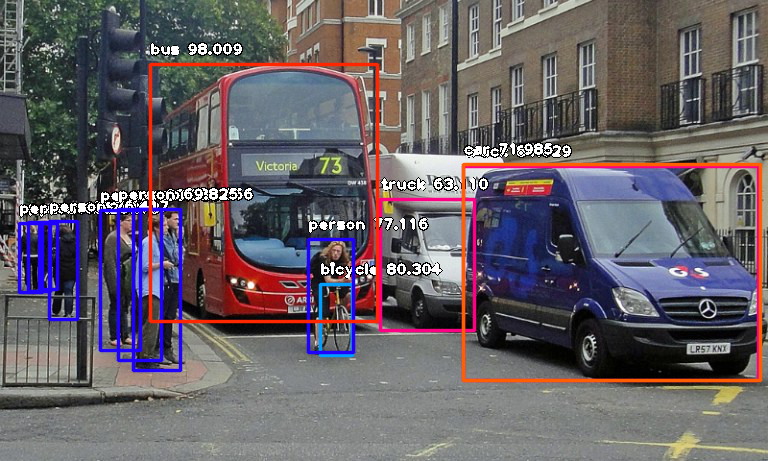
\includegraphics[width=11cm]{Obrazy/rozpoznawanieObiektow}
        \caption{Przykład rozpoznawania obiektów na zdjęciu ulicy. \cite{rozpoznawanieObiektow}}.
        \label{fig.rozpoznawanieObiektow}
    \end{figure}

    Można znaleźć wiele witryn internetowych, które udostępniają interfejsy programistyczne umożliwiające zaimplementowanie
    rozpoznawania wieku z obrazu.
    Istnieją algorytmy przetwarzania obrazu, które oprócz wieku wyznaczają z pewnym prawdopodobieństwem płeć danej osoby.
    Oprócz płci mogą one także wyznaczać
    wyraz twarzy oraz czy dana osoba posiada okulary.

    Z weryfikacją wieku danej osoby można się spotkać przed wejściem do niektórych miejsc np. klub nocny. Większość osób
    musi okazać ważny dowód osobisty.
    Co generuje duże kolejki do wejścia. Aplikację analizujące wiek na podstawie obrazu twarzy z kamery, przed wejściem
    do takich miejsc znacząco usprawniłyby weryfikację wieku.
    Rozpoznawanie wieku może być wykorzystywane przy analizie średniego wieku ludzi w jakimś miejscu np. podczas demonstracji.

    Wiele gier posiada treści nieodpowiednie dla młodszych użytkowników. Możliwe jest stosowanie technologii wykrywania
    wieku użytkownika przed udostępnieniem mu treści, która wymaga odpowiedniego wieku.

    Można znaleźć o wiele więcęj potencjalnych zastosowań przetwarzania obrazu oraz rozpoznawania wieku na podstawie
    tekstury (obrazu) twarzy. Z biegiem lat z pewnością będzie można zauważyć dalszy rozwój tej dziedziny.

    \section{Cel i zakres pracy}
    Celem pracy magisterskiej jest stworzenie prostego programu do rozpoznawania wieku na podstawie tekstury twarzy.

    Zakres pracy obejmuje:
    \begin{itemize}
        \item Wybór bazowej metody wyznaczania wieku
        \item Stworzenie kilku modyfikacji bazowej metody
        \item Opis algorytmów każdej z metod wyznaczania wieku
        \item Porównanie wszystkich metod i wybór najlepszej
    \end{itemize}

    \chapter{Przegląd metod wyznaczania wieku}
    \section{Metoda a}
    \section{Metoda b}
    \section{Metoda wrinkle feature}

    \chapter{Metoda bazowa - wrinkle feature}

    \section{Metoda wykrywania twarzy}
    \section{Wyznaczanie stref}
    \section{Wykrywanie zmarszczek - detektor Canny}
    \section{Wyliczanie wrinkle feature}
    \section{Algorytm trenowania}
    \section{Grupowanie danych - FCM}

    \subsection{Wstęp do grupowania danych}
    \subsection{Metoda FCM}

    \section{Wyznaczanie wieku}


    \chapter{Modyfikacje metody bazowej}

    \section{Odjęcie wybranej strefy}

    \subsection{Zmiana algorytmu względem metody bazowej}

    \section{Zastosowanie metody HOG}
    \subsection{Opis algorytmu HOG}
    \subsection{Zastosowanie w projekcie}

    \section{Metoda HOG oraz grupowanie KNN}
    \subsection{Grupowanie KNN}
    \subsection{Zastosowanie w projekcie}

    \chapter{Badania}

    \chapter{Podsumowanie}



    %%%%%%%%%%%%%%%%%%%%%%%%%%%%%%%%%%%%%%%%%%
    \backmatter
    \pagenumbering{Roman}
    \stepcounter{stronyPozaNumeracja}
    \setcounter{page}{\value{stronyPozaNumeracja}}

    \pagestyle{tylkoNumeryStron}

    %%%%%%%%%%% bibliografia %%%%%%%%%%%%
    \bibliographystyle{plplain}
    \bibliography{bibliografia}

    %%%%%%%%%  DODATKI %%%%%%%%%%%%%%%%%%%

    \begin{appendices}


        \chapter*{Dokumentacja techniczna}

        \chapter*{Spis skrótów i symboli}

        \begin{itemize}
            \item[DNA] kwas deoksyrybonukleinowy (ang. \ang{deoxyribonucleic acid})
            \item[MVC] model -- widok -- kontroler (ang. \ang{model--view--controller})
            \item[$N$] liczebność zbioru danych
            \item[$\mu$] stopnień przyleżności do zbioru
            \item[$\mathbb{E}$] zbiór krawędzi grafu
            \item[$\mathcal{L}$] transformata Laplace'a
        \end{itemize}




        \chapter*{Zawartość dołączonej płyty}

        Do pracy dołączona jest płyta CD z~następującą zawartością:
        \begin{itemize}
            \item praca w~formacie \texttt{pdf},
            \item źródła programu,
            \item zbiory danych użyte w~eksperymentach.
        \end{itemize}

        \listoffigures
        \listoftables

    \end{appendices}


\end{document}


%% Finis coronat opus.